%package list
\documentclass{article}
\usepackage[top=3cm, bottom=3cm, outer=3cm, inner=3cm]{geometry}
\usepackage{multicol}
\usepackage{graphicx}
\usepackage{url}
%\usepackage{cite}
\usepackage{hyperref}
\usepackage{array}
\usepackage{bookmark}
%\usepackage{multicol}
\newcolumntype{x}[1]{>{\centering\arraybackslash\hspace{0pt}}p{#1}}
\usepackage{natbib}
\usepackage{pdfpages}
\usepackage{multirow}
\usepackage[normalem]{ulem}
\useunder{\uline}{\ul}{}
\usepackage{xcolor}

%\usepackage{booktabs}
\usepackage[labelformat=empty]{caption}
\usepackage{subcaption}
\usepackage{float}
\usepackage{array}
\usepackage{minted}

\setminted{fontsize=\small,numbers=left,autogobble}
\newenvironment{block}{\captionsetup{type=listing}}{}

\newcolumntype{M}[1]{>{\centering\arraybackslash}m{#1}}
\newcolumntype{N}{@{}m{0pt}@{}}

% para el codigo fuente
\usepackage{listings}
\usepackage{color, colortbl}
\definecolor{dkgreen}{rgb}{0,0.6,0}
\definecolor{gray}{rgb}{0.5,0.5,0.5}
\definecolor{mauve}{rgb}{0.58,0,0.82}
\definecolor{codebackground}{rgb}{0.95, 0.95, 0.92}
\definecolor{tablebackground}{rgb}{0.8, 0, 0}

\lstset{frame=tb,
	language=bash,
	aboveskip=3mm,
	belowskip=3mm,
	showstringspaces=false,
	columns=flexible,
	basicstyle={\small\ttfamily},
	numbers=none,
	numberstyle=\tiny\color{gray},
	keywordstyle=\color{blue},
	commentstyle=\color{dkgreen},
	stringstyle=\color{mauve},
	breaklines=true,
	breakatwhitespace=true,
	tabsize=3,
	backgroundcolor= \color{codebackground},
}

%Comando
\newcommand{\itemEmail}{mjarama@unsa.edu.pe}
\newcommand{\itemStudent}{Mariel Alisson Jara Mamani}
\newcommand{\itemStudentShort}{Mariel Jara}
\newcommand{\itemCourse}{Programación Web 2}
\newcommand{\itemCourseCode}{1702122}
\newcommand{\itemSemester}{I}
\newcommand{\itemUniversity}{Universidad Nacional de San Agustín de Arequipa}
\newcommand{\itemFaculty}{Facultad de Ingeniería de Producción y Servicios}
\newcommand{\itemDepartment}{Departamento Académico de Ingeniería de Sistemas e Informática}
\newcommand{\itemSchool}{Escuela Profesional de Ingeniería de Sistemas}
\newcommand{\itemAcademic}{2023 \- B}
\newcommand{\itemInput}{Del 19 Junio 2024}
\newcommand{\itemOutput}{Al 23 Junio 2024}
\newcommand{\itemPracticeNumber}{08}
\newcommand{\itemTheme}{Django: ORM, PDFs y correos electrónicos}
\renewcommand{\contentsname}{Laboratorio \itemPracticeNumber}
%%%%%%%%%%%%%%%%%%%%%%%%%%%%%%%%%%%%%%%%%%%%%%%%%%%%%%%%%%%%%%%%%%%%%%%%%%%%
%%%%%%%%%%%%%%%%%%%%%%%%%%%%%%%%%%%%%%%%%%%%%%%%%%%%%%%%%%%%%%%%%%%%%%%%%%%%

\usepackage[utf8]{inputenc}
\renewcommand{\figurename}{Figura}
\renewcommand{\refname}{Referencias}
\renewcommand{\tablename}{Tabla} %esto no funciona cuando se usa babel
\AtBeginDocument{%
\renewcommand\tablename{Tabla}
\setlength{\headheight}{40.51407pt}
}

\usepackage{fancyhdr}
\pagestyle{fancy}
\fancyhf{}
\setlength{\headheight}{30pt}
\renewcommand{\headrulewidth}{1pt}
\renewcommand{\footrulewidth}{1pt}
\fancyhead[L]{\raisebox{-0.2\height}{
\includegraphics[width=3cm]{img/episunsa.png}}}
\fancyhead[C]{\fontsize{7}{7}\selectfont	\itemUniversity \\ \itemFaculty \\ \itemDepartment \\ \itemSchool \\ \textbf{\itemCourse}}
\fancyhead[R]{\raisebox{-0.2\height}{
\includegraphics[width=1.2cm]{img/logo_abet.png}}}
\fancyfoot[L]{\itemStudentShort}
\fancyfoot[C]{\itemCourse}
\fancyfoot[R]{Página \thepage}

\begin{document}

\vspace*{10px}

\begin{center}
	\fontsize{17}{17} \textbf{ Informe de Laboratorio \itemPracticeNumber}
\end{center}
\centerline{\textbf{\Large Tema: \itemTheme}}
%\vspace*{0.5cm}	

\begin{flushright}
	\begin{tabular}{|M{2.5cm}|N|}
		\hline
		\rowcolor{tablebackground}
		\color{white} \textbf{Nota} \\
		\hline
		\\[30pt]
		\hline
	\end{tabular}
\end{flushright}

\begin{table}[H]
	\begin{tabular}{|M{5.4cm}|M{4.0cm}|M{4.7cm}|}
		\hline
		\rowcolor{tablebackground}
		\color{white} \textbf{Estudiante(s)} & \color{white}\textbf{Escuela} & \color{white}\textbf{Asignatura}                                        \\
		\hline
		{\itemStudent \par \itemEmail}       & \itemSchool                   & {\itemCourse \par Semestre: \itemSemester \par Código: \itemCourseCode} \\
		\hline
	\end{tabular}
\end{table}

\begin{table}[H]
	\begin{tabular}{|M{4.7cm}|M{4.7cm}|M{4.7cm}|}
		\hline
		\rowcolor{tablebackground}
		\color{white}\textbf{Laboratorio} & \color{white}\textbf{Tema} & \color{white}\textbf{Duración} \\
		\hline
		\itemPracticeNumber               & \itemTheme                 & 04 horas                       \\
		\hline
	\end{tabular}
\end{table}

\begin{table}[H]
	\begin{tabular}{|M{4.7cm}|M{4.7cm}|M{4.7cm}|}
		\hline
		\rowcolor{tablebackground}
		\color{white}\textbf{Semestre académico} & \color{white}\textbf{Fecha de inicio} & \color{white}\textbf{Fecha de entrega} \\
		\hline
		\itemAcademic                            & \itemInput                            & \itemOutput                            \\
		\hline
	\end{tabular}
\end{table}
\pagebreak

\tableofcontents
\pagebreak


%%%%%%%%%%%%%%%%%%%%%%%%%%%%%%%%%%%%%%%%%%%%%%%%%%%%%%%%%%%%%%%%%%%%%%
\section{Tarea}
\begin{itemize}
	\item Deberán replicar la actividad de los videos donde se trabaja con Relacion de uno a muchos, de muchos a muchos, impresión de pdfs y envio de emails; y adecuarla a un proyecto en blanco Django.
	\item Para ello crear una carpeta dentro del proyecto github colaborativo con el docente, e informar el link donde se encuentra.
	\item Eres libre de agregar CSS para decorar tu trabajo.
	\item \textbf{Observaciones:}
	      \begin{itemize}
		      \item Ya sabes que el trabajo con Git es obligatorio. Revisa los videos entregados.
		      \item Cada commit debe ser realizado con un mensaje descriptivo que estuvo siguiendo. Si los mensajes no son claros respecto al código “commiteado” tendrá menos calificación.
	      \end{itemize}
\end{itemize}
\pagebreak
%%%%%%%%%%%%%%%%%%%%%%%%%%%%%%%%%%%%%%%%%%%%%%%%%%%%%%%%%%%%%%%%%%%%%%
\section{Commits}
\begin{figure}[H]
	\centering
	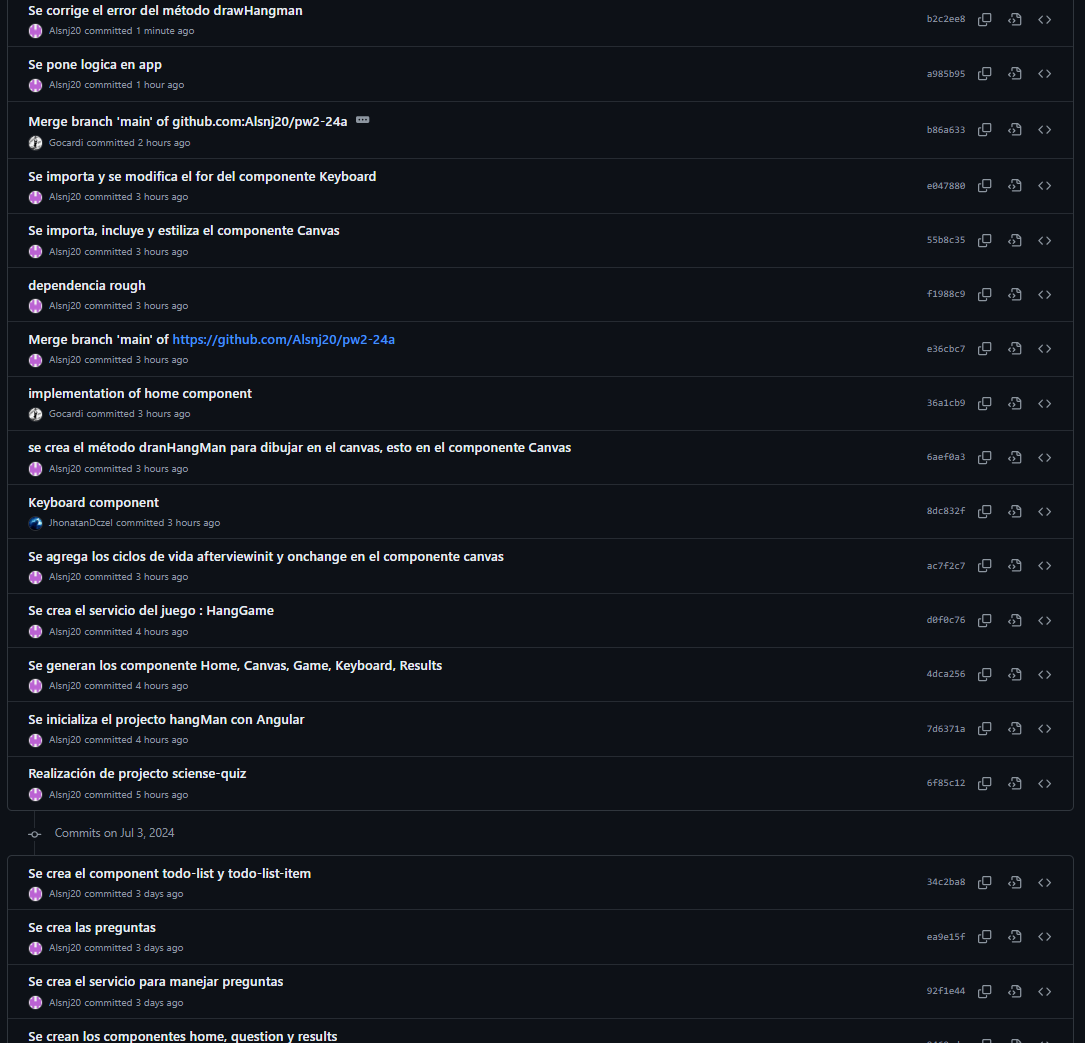
\includegraphics[width=0.9\textwidth,keepaspectratio]{img/commits.png}
	\caption{Lista de commits.}
\end{figure}
\pagebreak
\section{Equipos y materiales utilizados}
\begin{itemize}
	%%%%%%%%%%%%%%%%%%%%%%%%%%%%%%%%%%%%%%%%%%%%%%%%%%%%%%%%%%%%%%%%%%%%%%
	\item Cuenta en GitHub con el correo institucional.
	\item Sistema Operativo Microsoft Windows 10
	\item Visual Studio Code
	\item Git
	\item Windows PowerShell
	\item Python
	\item Navegador Mozilla Firefox
	      %%%%%%%%%%%%%%%%%%%%%%%%%%%%%%%%%%%%%%%%%%%%%%%%%%%%%%%%%%%%%%%%%%%%%%
\end{itemize}
\pagebreak

\section{URL del repositorio en GitHub}
\begin{itemize}
	\item \url{https://github.com/Alsnj20/pw2-24a/tree/main/lab09}
\end{itemize}
\pagebreak
\section{Estructura de laboratorio \itemPracticeNumber}
\begin{itemize}
	\item El contenido que se entrega en este laboratorio es el siguiente:
\end{itemize}
\begin{lstlisting}{language=bash}
lab08/
	|--Course_Management_System/
		|--systemM/
			|--migrations/
			|--templates/
				|--css/
					|--form-page.css
					|--lists.css
					|--nav.css
				|--pdf/
					|--certified.html
					|--generate_certified.html
					|--index.html
					|--invoice.html
					|--list_courses.html
					|--list_students.html
					|--nav.html
					|--register_course.html
					|--register_student.html
					|--send_message.html
			|--__init__.py
			|--admin.py
			|--apps.py
			|--forms.py
			|--models.py
			|--renderers.py
			|--tests.py
			|--urls.py
			|--views.py
		|--system/
	|--relations_examples/
	|--email_example/
	|--print_pdfs/
|--Latex/
		|--linopinto_pw2_24a_lab08.tex
		|--linopinto_pw2_24a_lab08.pdf
		|--img/
			 |--commits.png
			 |--r1operaciones.png
			 |--r2operations.png
			 |--r1tabla1.png
			 |--r1tabla2.png
			 |--r2tabla1.png
			 |--r2tabla2.png
			 |--r2tabla3.png
			 |--send_email.png
			 |--print_pdf.png
			 |--registerStudent.png
			 |--registerSBD.png
			 |--registerCourse.png
			 |--registerCBD.png
			 |--relation.png
			 |--listStudents.png
			 |--listCourses.png
			 |--sendMessage.png
			 |--certificado.png
|--.gitignore
\end{lstlisting}
\section{Rúbrica}

\section{Referencias}
\begin{itemize}
	\item \url{https://github.com/}
	\item \url{https://git-scm.com/}
	\item \url{https://www.w3schools.com/python/}
\end{itemize}

\pagebreak
\bibliographystyle{apalike}
\bibliographystyle{IEEEtranN}
\bibliography{bibliography}

\end{document}